\achapter{3}{Row Echelon Forms} \label{sec:row_echelon_forms}

\vspace*{-17 pt}
\framebox{
\parbox{\dimexpr\linewidth-3\fboxsep-3\fboxrule}
{\begin{fqs}
\item What is the row echelon form of a matrix?
\item What is the procedure to obtain the row echelon form of any matrix?
\item What is the reduced row echelon form of a matrix?
\item What is the procedure to obtain the reduced row echelon form of any matrix?
\item What do the echelon forms of the augmented matrix for a linear system tell us about the solutions to the system?
\end{fqs}}}% \hspace*{3 pt}}

\vspace*{13 pt}

\csection{Application: Balancing Chemical Reactions}

Linear systems have applications in chemistry when balancing chemical equations. When a chemical reaction occurs, molecules of different substances combine to create molecules of other substances. Chemists represent such reactions with chemical equations. To balance a chemical equation means to find the number of atoms of each element involved that will preserve the number of atoms in the reaction. 
As an example, consider the chemical equation
\begin{equation}
\text{C}_2\text{H}_6 + \text{O}_2 \to \text{CO}_2 + \text{H}_2\text{O}. \label{eq:reaction1}
\end{equation}
This equation asks about what will happen when the chemicals ethane ($\text{C}_2\text{H}_6$) and oxygen ($\text{O}_2$), called the \emph{reactants} of the reaction, combine to produce carbon dioxide ($\text{CO}_2$) and water ($\text{H}_2\text{O}$), called the \emph{products} of the reaction (note that oxygen gas is \emph{diatomic}, so that oxygen atoms are paired). The arrow indicates that it is the reactants that combine to form the products. Any chemical reaction has to obey the Law of Conservation of Mass that says that mass can neither be created nor destroyed in a chemical reaction. Consequently, a chemical reaction requires the same number of atoms on both sides of the reaction. In other words, the total mass of the reactants must equal the total mass of the products. In reaction (\ref{eq:reaction1}) the chemicals involved are made up of carbon (C), hydrogen (H), and oxygen (O) atoms. To balance the equation, we need to know how many molecules of each chemical are combined to preserve the number of atoms of C, H, and O. This can be done by setting up a linear system of equations of the form 
\begin{alignat*}{5}
{2}x_1 	&{}		&{}		&{}-{}	&{}x_3	&{}		&{} 			&{}={}	& \ 0&{}   \\
{6}x_1	&{} 		&{} 		&{}		&{}		&{}-{}	&{2}x_4 	&{}={} 	& \ 0&{} \\
{}			&{}		&{2}x_2	&{}-{} 	&{2}x_3	&{}-{}	&{}x_4		&{}={} 	& \ 0&{,}
\end{alignat*}
where $x_1$, $x_2$, $x_3$, and $x_4$ represent the number of molecules of $\text{C}_2\text{H}_6$,  $\text{O}_2$,  $\text{CO}_2$, and $\text{H}_2\text{O}$, respectively, in the reaction and then solving the system. Specific details can be found at the end of this section. 

\csection{Introduction}

In the previous sections, we identified operations on a given linear system with corresponding equivalent operations on the matrix representations which simplify the system and its matrix representation without changing the solutions of the system. Our end goal was to obtain a system which could be solved using back substitution, such as 

\begin{alignat*}{4}
{}x_1 	&{}-{} 	&{}x_2 	&{}+{} 	&{}x_3 &{}={}	&0&{}   \\
{}			&{} 		&{6}x_2 &{}-{}	&{}x_3 &{}={} 	&8&{} \\
{}			&{}		&{}		&{}	 	&{}x_3 &{}={} 	&1&{.} 
\end{alignat*}
The augmented matrix for this system is
\[ \left[ \begin{array}{crr|c} 1 &-1 &1 &0 \\ 0& 6 &-1 &8 \\ 0&0 &1 &1 \end{array} \right]. \]
The matrices of linear systems which can be solved via back substitution are said to be in \emph{row echelon form} (or simply \emph{echelon form}). We will define the properties of matrices in this form precisely in this section. Our goal will be to prescribe a precise procedure for converting any matrix to an equivalent one in row echelon form without having to convert back to the system representation.

\begin{pa} \label{pa:1_c}  We want to determine a suitable form for an augmented matrix that can be obtained from row operations so that it is straightforward to find the solutions to the system. We begin with some examples.

\be
\item Write the linear system corresponding to each of the following augmented matrices. Use the linear system to determine which systems have their variables eliminated completely in the forward direction, or equivalently determine for which systems the next step in the solution process is back substitution (possibly using free variables). Explain your reasoning. You do not need to solve the systems. 
	\begin{enumerate}[i.]
	\begin{minipage}{2.0in}
	\item $\ds \left[ \begin{array}{rrc|r} 1 & -1 & 2 & -2 \\ 0 & 1 & 2& -1 \\ 0 & 0 & 3 & 1   \end{array} \right]$
	\end{minipage}
	\begin{minipage}{2.0in}
	\item $\ds \left[ \begin{array}{crc|r} 1 & 1 & 0 & -2 \\ 0 & 1 & 0 & 3  \\ 0 & 0 & 0& 0 \end{array} \right]$
	\end{minipage}
	
	\begin{minipage}{2.0in}
	\item $\ds \left[ \begin{array}{ccc|c} 1 & 1 & 1 & 2 \\ 1 & 2 & 2 & 2  \\ 0 & 0 & 2& 2 \end{array} \right]$
	\end{minipage}
	\begin{minipage}{2.0in}
	\item $\ds \left[ \begin{array}{ccr|r} 0 & 1 & 1 & 2 \\ 0 & 0 & 3 & 3 \\ 0 & 0 & -2& -2 \end{array} \right]$
	\end{minipage}
	
	\end{enumerate}
	
	\item Shown below are two row reduced forms of the system 
	\begin{alignat*}{5}
{2}x_1 	&{}		&{}		&{}-{}	&{}x_3	&{}		&{} 			&{}={}	& \ 0&{}   \\
{6}x_1	&{} 		&{} 		&{}		&{}		&{}-{}	&{2}x_4 	&{}={} 	& \ 0&{} \\
{}			&{}		&{2}x_2	&{}-{} 	&{2}x_3	&{}-{}	&{}x_4		&{}={} 	& \ 0&{.}
\end{alignat*} 
Of the systems that correspond to these augmented matrices, which is easier to solve and why?
\[\left[ \begin{array}{cccr|c} 2 & 0 & -1 & 0 & 0 \\ 0 & 2 & -2 & -1 & 0 \\ 0 & 0 & 3 & -2 & 0 \end{array} \right] \hspace{0.25in} \left[ \renewcommand{\arraystretch}{1.4} \begin{array}{cccr|c} 1 & 0 & 0 & -\frac{1}{3} & 0 \\ 0 & 1 & 0 & -\frac{7}{6} & 0 \\ 0 & 0 & 1 & -\frac{2}{3} & 0 \end{array} \right]\]	

\ee

\end{pa}


\csection{The Echelon Forms of a Matrix}

In the previous sections we saw how to simplify a linear system and its matrix representation via the elimination method without changing the solution set. This process is more efficient when performed on the matrix representation rather than on the system itself. Furthermore, the process of applying row operations to any augmented matrix is one that can be automated. In order to write an algorithm that can be used with any size augmented matrix to the extent that it can be applied even by a computer program, it is necessary to have a consistent procedure and a stopping point for the simplification process. The two main properties that we want the simplified augmented matrix to satisfy are that it should be easy to see if the system has solutions from the simplified matrix, and in cases when there are solutions, the general form of the solutions can be easily found. Hence the topic of this section is to define the process of elimination completely and generally.

We begin by discussing the \emph{row echelon} or, simply, \emph{echelon} form of a matrix. We know that the forward phase of the elimination on a linear system produces a system which can be solved by back substitution. The matrix representation of such a simplified system is said to be in \emph{row echelon} or simply \emph{echelon} form. Note that matrices in this form have the first nonzero entry in each row to the right of and below the first nonzero entry in the preceding row. Our next step is to formally describe this form -- one that you tried to explain in problem 3 of Preview Activity \ref{pa:1_c}. 



\begin{definition} A rectangular matrix is in \textbf{row echelon form}\index{row echelon form} (or simply \textbf{echelon form}) if it has the following properties:
        \begin{enumerate}
        \item All nonzero rows are above any rows of all zeros.
        \item Each \textbf{pivot}\index{pivot} (the first non-zero entry reading from left to right) in a row is in a column to the right of the pivot of the row above it.
        \end{enumerate}
\end{definition}

A pivot is also called a \emph{leading entry}\index{leading entry of a row} of a row. Note that properties (1) and (2) above imply that all entries in a column below a pivot are zeros. It can be shown that the positions of these pivots, called \textbf{pivot positions}\index{pivot positions}, are unique and tell us quite a bit about a matrix and the solutions of the linear system it corresponds to. The columns that the pivots are in, called \textbf{pivot columns}\index{pivot column}, will also have useful properties as we will see soon.

\begin{reflect} Compare the row echelon form of an augmented matrix to the corresponding system. Do you clearly see the correspondence between the requirements of the row echelon form and the properly eliminated variables in the system? Can you quickly come up with a system which will be in row echelon form when represented in augmented matrix form? Can you modify the standard row echelon form definition to cover cases where the elimination process eliminates the variables from last to first? For example, in a system with three equations in three unknowns, the last variable, say $x_3$, can be eliminated from the second equation, and the last two variables, say $x_2, x_3$ can be eliminated from the last equation. How would you define this modified row echelon form for a general system with this modified elimination process?
\end{reflect}



Once an augmented matrix is in row echelon form, we can use back substitution to solve the corresponding system. However, we can make solving much easier with just a little more elimination work. 

Row operations are easy to apply, so if we are inclined, there is no reason to stop at the row echelon form. For example, starting with the following matrix 
\[\left[ \begin{array}{crcr|r} 2&-1&2&2&7 \\ 0&1&3&-1&-1 \\ 0&0&0&2&4 \end{array} \right]\]
in row echelon form, we could take the row operations even farther and avoid the process of back substitution altogether. First, we multiply the last row by $1/2$ to simplify that row:
\[\begin{array}{c} \text{ }\\ \text{ }\\ \text{\scriptsize $\frac{1}{2} R_3 \to R_3$} \end{array} \left[ \begin{array}{crcr|r} 2&-1&2&2&7 \\ 0&1&3&-1&-1 \\ 0&0&0&1&2 \end{array} \right].\]
Then we use the third row to eliminate entries above the third pivot:
\[\begin{array}{c} \text{\scriptsize $R_1-2R_3 \to R_1$}\\ \text{\scriptsize $R_2+R_3 \to R_2$} \\ \text{ }\end{array}  \left[ \begin{array}{crcr|r} 2&-1&2&0&3 \\ 0&1&3&0&1 \\ 0&0&0&1&2 \end{array} \right].\]
We can continue in this manner (we call this process \emph{backward elimination}) to make 0 all of the entries above the pivots (one in the second column, and one in the fourth) with the pivots being 1, to ultimately obtain the equivalent augmented matrix
\[\left[ \begin{array}{crcr|r} 1&0&1&0&2 \\ 0&1&3&0&1 \\ 0&0&0&1&2 \end{array} \right].\]
The system corresponding to this augmented matrix is
\begin{alignat*}{5}
{}x_1 	&{}	 	&{}		&{}+{}	&{}x_3		&{\hspace{0.2in}}		&{} 		&{}={}	& \ 2   \\
{}			&{} 		&{}x_2 	&{}+{}	&{3}x_3		&{ }							&{} 		&{}={} 	& \ 1 \\
{}			&{}		&{}		&{}	 	&{}			&{ }							&{}x_4	&{}={} 	& \ 2
\end{alignat*}
so we can just directly read off the solution to the system: $x_3$ free and $x_1=2-x_3, x_2=1-3x_3, x_4=2$. This final row reduced form makes solving the system very easy, and this form is called the \emph{reduced row echelon} form. 
 


\begin{definition} A rectangular matrix is in \textbf{reduced row echelon form}\index{row echelon form!reduced} (or \textbf{reduced echelon form}) if the matrix is in row echelon form and 
        \begin{enumerate}
        \item[(3)] The pivot in each nonzero row is 1.
        \item[(4)] Each pivot is the only nonzero entry in its column.
        \end{enumerate}
\end{definition}



In short, the reduced row echelon form of a matrix is a row echelon form in which all the pivots are 1 and any entries \underline{below and above} the pivots are 0.

If we use either of these two row echelon forms, solving the original system becomes straightforward and, as a result, these matrix forms are stopping points for the row operation algorithm to solve a system. It is also very easy to write a computer program to perform row operations to obtain and row echelon or reduced row echelon form of the matrix, making hand computations unnecessary. We will discuss this shortly. 
 
\begin{reflect}Compare the reduced row echelon form of an augmented matrix to the corresponding system. Do you clearly see the correspondence between the requirements of the reduced row echelon form and the way the variables appear in the equations in the system? Can you quickly come up with a system which will be in reduced row echelon form when represented in augmented matrix form?
\end{reflect}



\begin{note} We have used the elimination method on augmented matrices so far. However, the elimination method can be applied on just the coefficient matrix, or other matrices that will arise in other contexts, and will provide useful information in each of those cases. Therefore, the row echelon form and reduced row echelon form is defined for \underline{any matrix}, and from now on, a matrix will be a general matrix unless explicitly specified to be an augmented matrix.
\end{note} 




\begin{activity} \label{act:1_c_1} Identify which of the following matrices is in row echelon form (REF) and/or reduced row echelon form (RREF). For those in row and/or reduced row echelon form, identify the pivots clearly by circling them. For those that are not in a given form, state which properties the matrix fails to satisfy. 

\ba
\begin{minipage}{1.75in}
 \item $\left[ \begin{array}{ccrc} 2 & 4 & -3 & 6 \\ 0 & 0 & 0 & 7 \end{array} \right]$ 
\end{minipage}
\begin{minipage}{1.5in}
\item $\left[ \begin{array}{cc} 1 & 0  \\ 0 & 1 \end{array} \right]$ 
\end{minipage}
\begin{minipage}{1.5in}
\item $\left[ \begin{array}{cccc} 0 & 1 & 2 & 3 \\ 0 & 0 & 1 & 0 \\ 0 & 1 & 0 & 5 \end{array} \right]$ 
\end{minipage} 

\begin{minipage}{1.75in}
\item $\left[ \begin{array}{cccc} 1 & 2 & 3 & 4 \\ 0 & 0 & 0 & 0 \\ 0 & 0 & 0 & 0 \end{array} \right]$ 
\end{minipage}
\begin{minipage}{1.5in}
\item $\left[ \begin{array}{cc} 0 & 0 \\ 0 & 0 \end{array} \right]$ 
\end{minipage}
\ea 

\end{activity}


\csection{Determining the Number of Solutions of a Linear System}

Consider the system
\begin{alignat*}{5}
{}x_1 	&{+}		&{2}x_2		&{}-{}	&{}x_3	&{}		&{} 			&{}={}	& \ 0&{}   \\
{}		&{} 		&{}x_2 		&{}		&{}		&{}-{}	&{}x_4 	&{}={} 	& \ 2&{} \\
{}			&{}		&{}	&{}{} 			&{}x_3	&{}-{}	&{2}x_4		&{}={} 	& \ 4&{.}
\end{alignat*}
The augmented matrix for this system is 
\[\left[ \begin{array}{ccrr|c} 1 & 2 & -1 & 0 & 0 \\ 0 & 1 & 0 & -1 & 2 \\ 0 & 0 & 1 & -2 & 4 \end{array} \right].\]
Note that this matrix is already in row echelon form. The reduced row echelon form of this augmented matrix is 
\begin{equation} \label{eq:Ex_rref}
\left[ \begin{array}{cccr|c} 1 & 0 & 0 & 0 & 0 \\ 0 & 1 & 0 & -1 & 2 \\ 0 & 0 & 1 & -2 & 4 \end{array} \right].
\end{equation}

Since there are leading 1s in the first three columns, we can use those entries to write $x_1$, $x_2$, and $x_3$ in terms of $x_4$. We then choose $x_4$ to be arbitrary and write the remaining variables in terms of $x_4$. Let $x_4 = t$. Solving the third equation for $x_3$ gives us $x_3 = 4+2t$. The second equation shows that $x_2 = 2+t$, and the first that $x_1 = 0$. Each value of $t$ provides a solution to the system, so our system has infinitely many solutions. These solutions are 
\[x_1 = 0, \ x_2 = 2+t, \ x_3 = 4+2t, \ \text{ and } \ x_4 = t,\]
where $t$ can have any value. 

\begin{activity} \label{act:1_c_2} We have seen examples of systems with no solutions, one solution, and infinitely many solutions. As we will see in this activity, we can recognize the number of solutions to a system by analyzing the pivot positions in the augmented matrix of the system.  
    \ba
    \item Write an example of an augmented matrix in row echelon form so that the last column of the (whole) matrix is a pivot column. What is the system of equations corresponding to your augmented matrix? How many solutions does your system have? Why? 
		

    \item Consider the reduced row echelon form (\ref{eq:Ex_rref}). Based on the columns of this matrix, explain how we know that the system it represents is consistent. 

	\item The system with reduced row echelon form (\ref{eq:Ex_rref}) is consistent. What is it about the columns of the coefficient matrix that tells us that this system has infinitely many solutions? 

     \item Suppose that a linear system is consistent and that the coefficient matrix has $m$ rows and $n$ columns. 
		\begin{enumerate}[i.]
		\item If every column of the coefficient matrix is a pivot column, how many solutions must the system have? Why? What relationship must exist between $m$ and $n$? Explain.
		\item If the coefficient matrix has at least one non-pivot column, how many solutions must the system have? Why? 
		\end{enumerate}

    \ea

\end{activity}


When solving a linear system of equations, the free variables can be chosen arbitrarily and we can write the basic variables in terms of the free variables. Therefore, the existence of a free variable leads to infinitely many solutions for consistent systems. However, it is possible to have a system with free variables which is inconsistent. (Can you think of an example?)

\csection{Producing the Echelon Forms}

In this part, we consider the formal process of creating the row and reduced row echelon forms of matrices. The process of creating the row echelon form is the equivalent of the elimination method on systems of linear equations.

\begin{activity} Each of the following matrices is at most a few steps away from being in the requested echelon form. Determine what row operations need to be completed to turn the matrix into the required form.

\ba
\begin{minipage}{2.4in}
\item Turn into REF: $\left[ \begin{array}{cc} 0 & 2 \\ 2 & 1 \end{array} \right]$
\end{minipage} 
\begin{minipage}{2.0in}
\item Turn into REF: $\left[ \begin{array}{cc} 1 & 2 \\ 2 & 5 \end{array} \right]$
\end{minipage}

\begin{minipage}{2.4in}
\item Turn into RREF: $\left[ \begin{array}{ccc} 2 & 0 &0 \\ 0 & 3 &0 \\ 0&0&1\end{array} \right]$
\end{minipage}
\begin{minipage}{2.0in}
\item Turn into RREF: $\left[ \begin{array}{cr} 1& -1 \\ 0 & 1 \end{array} \right]$
\end{minipage}

\begin{minipage}{2.4in}
\item Turn into RREF: $\left[ \begin{array}{cc} 1& 1 \\ 0 & 2 \end{array} \right]$
\end{minipage}
\begin{minipage}{2.0in}
\item Turn into RREF: $\left[ \begin{array}{ccr} 1& 0 &-1 \\ 0 & 1 &3 \\ 0&0&2 \end{array} \right]$
\end{minipage}
\ea

\end{activity}

The complete process of applying row operations to reduce an augmented matrix to a row or reduced row echelon form can be expressed as a recursive process in an algorithmic fashion, making it possible to program computers to solve linear systems. Here are the steps to do so: 

\begin{description}
\item[Step 1:] Begin with the leftmost nonzero column (if there is one). This will be a pivot column. 

\item[Step 2:] Select a nonzero entry in this pivot column as a pivot. If necessary, interchange rows to move this entry to the first row (this entry will be a pivot).

\item[Step 3:] Use row operations to create zeros in all positions below the pivot.

\item[Step 4:] Cover (or ignore) the row containing the pivot position and cover all rows, if any, above it. Apply steps 1-3 to the submatrix that remains. Repeat the process until there are no more nonzero rows to modify.
\end{description}

To obtain the reduced row echelon form we need one more step.

\begin{description}
\item[Step 5:] Beginning with the rightmost pivot and working upward and to the left, create zeros above each pivot. If a pivot is not 1, make it 1 by an appropriate row multiplication.
\end{description}

The algorithm described in steps 1-4 will produce the row echelon form of the matrix. This algorithm is called \emph{Gaussian elimination}. When we add step 5 to produce the reduced row echelon form, the algorithm is called \emph{Gauss-Jordan elimination}.



\begin{activity} \label{act:1_c_3} Consider the matrix $\left[ \begin {array}{rrcr} 0&2&4&1\\ -1&3&0&6 \\ 0&4&8&2\\ 1&-3&0&-2\end {array}  \right]$. 
	\ba
	\item Perform Gaussian elimination to reduce the matrix to row echelon form. Clearly identify each step used. Compare your row echelon form to that of another group. Do your results agree? If not, who is right?
	
	
	
	\item Now continue applying row operations to obtain the reduced row echelon form of the matrix. Clearly identify each step. Compare your row echelon form to that of another group. Do your results agree? If not, who is right?
	
	
	
	\ea
\end{activity}



If we compare row echelon forms from Activity \ref{act:1_c_3}, it is likely that different groups or individuals produced different row echelon forms. That is because the row echelon form of a matrix is not unique. (Is the row echelon form ever unique?)

However, if row operations are applied correctly, then we will all arrive at the same reduced row echelon form in Activity \ref{act:1_c_3}:
\[\left[ \begin{array}{cccc} 1&0&6&0\\ 0&1&2&0 \\ 0&0&0&1\\ 0&0&0&0 \end{array}  \right].\]
It turns out that the reduced row echelon form of a matrix is unique. 

Two matrices who are connected by row operations are said to be \emph{row equivalent}.

\begin{definition} A matrix $B$ is \textbf{row equivalent}\index{row equivalent matrices} to a matrix $A$ if $B$ can be obtained by applying elementary row operations to $A$.
\end{definition}

Since every elementary row operation is reversible, if $B$ is row equivalent to $A$, then $A$ is also row equivalent to $B$. Thus, we just say that $A$ and $B$ are row equivalent. While the row echelon form of a matrix is not unique, it is the case that the reduced row echelon form of a matrix is unique. 

\begin{theorem}Every matrix is row equivalent to a unique matrix in reduced row echelon form.
\end{theorem}

The reduced row echelon form of a matrix that corresponds to a system of linear equations provides us with an equivalent system whose solutions are easy to find. As an example, consider the system 
\begin{alignat*}{5}
{} 		&{}	 	&{2}x_2	&{}+{}	&{4}x_3	&{}+{}	&{}x_4	&{}={}	& \ 0   \\
{-}x_1	&{}+{}	&{3}x_2	&{}		&{}		&{}+{}	&{6}x_4	&{}={} 	& \ 0 \\
{}			&{}		&{4}x_2	&{}+{} 	&{8}x_3	&{}+{}	&{2}x_4	&{}={} 	& \ 0 \\
{}x_1	&{}-{}	&{3}x_2	&{}	 	&{}		&{}-{}	&{2}x_4	&{}={} 	& \ 0 
\end{alignat*}
with augmented matrix 
\[\left[ \begin{array}{rrcr|c} 0&2&4&1&0 \\ -1&3&0&6&0 \\ 0&4&8&2&0 \\ 1&-3&0&-2&0 \end{array}  \right].\]
Notice that the coefficient matrix (the left hand side portion of the augmented matrix) of this system is same as the matrix we considered in Activity \ref{act:1_c_3}. Since we are augmenting with a column of zeros, no row operations will change those zeros in the augmented column. So the row operations applied in Activity \ref{act:1_c_3} will give us the reduced row echelon form of this augmented matrix as 
\[\left[ \begin{array}{cccc|c} 1&0&6&0&0\\ 0&1&2&0&0 \\ 0&0&0&1&0 \\ 0&0&0&0&0 \end{array} \right].\]
Note that the third column is not a pivot column. That means that the variable $x_3$ is a free variable. There are pivots in the other three columns of the coefficient matrix, so we can solve for $x_1$, $x_2$, and $x_4$ in terms of $x_3$. These variables are the basic variables. The third row of the augmented matrix tells us that $x_4=0$. The second row corresponds to the equation $x_2+2x_3 = 0$, and solving for $x_2$ shows that $x_2 = -2x_3$. Finally, the first row tells us that $x_1+6x_3 = 0$, so $x_1 = -6x_3$. Therefore, the general solution to this system of equations is 
\[x_1 = -6x_3, \ \ \ \ x_2 = -2x_3, \ \ \ \ x_3 \text{ is free}, \ \ \ \  x_4 = 0.\]
The fact that $x_3$ is free means that we can choose any value for $x_3$ that we like and obtain a specific solution to the system. For example, if $x_3=-1$, then we have the solution $x_1 = 6$, $x_2 = 2$, $x_3 = -1$, and $x_4 = 0$. Check this to be sure. 

\begin{activity}
Each matrix below is an augmented matrix for a linear system after elimination with variables $x_1, x_2, \ldots$ in that order. Identify the basic variables (if any) and free variables (if any). Then find the general solution (if there is a solution) expressing all variables in terms of the free variables. 
	\ba
	\begin{minipage}{1.5in}
	\item $\left[ \begin{array}{ccc|c} 1&0&2&1 \\ 0&3&1&0 \\ 0&0&0&0 \end{array} \right]$
	\end{minipage}
	\begin{minipage}{1.5in}
	\item $\left[ \begin{array}{ccr|c} 1&1&0&1 \\ 0&0&1&2 \\ 0&0&0&0 \end{array} \right]$
	\end{minipage}
	\begin{minipage}{1.5in}
	\item $\left[ \begin{array}{ccrc|c} 1&2&-1&1&1 \\ 0&1&0&2&1 \\ 0&0&0&0&0 \\ 0&0&0&0&0 \end{array} \right]$
	\end{minipage}

	\begin{minipage}{1.5in}
	\item $\left[ \begin{array}{ccr|c} 1&0&1&1 \\ 0&1&0&0 \\ 0&0&0&2 \end{array} \right]$
	\end{minipage}
	\begin{minipage}{1.5in}
	\item $\left[ \begin{array}{cc|c} 1&0&1 \\ 0&1&0 \\ 0&0&0 \end{array} \right]$
	\end{minipage}

\ea

\end{activity}


%\begin{reflect} For a system of equations with all right hand sides being 0, if the row operations keep those 0's in place, what does this mean in terms of whether the system has a solution or not? Is it possible for such a system to be inconsistent?
%\end{reflect}

Recall that in the previous section, we determined the criteria for when a system has a unique solution, or infinitely many solutions, or no solution. With the use of the row echelon form of the augmented matrix, we can rewrite these criteria as follows:

\begin{theorem} ~
\begin{enumerate}
\item A linear system is consistent if in the row echelon form of the augmented matrix representing the system no pivot is in the rightmost column. 
\item If a linear system is consistent and the row echelon form of the coefficient matrix does not have a pivot in every column, then the system has infinitely many solutions. 
\item If a linear system is consistent and there is a pivot in every column of the row echelon form of the coefficient matrix, then the system has a  unique solution.
\end{enumerate}
\end{theorem}






\begin{figure}[ht]
\begin{center}
\begin{minipage}{1.75in}
\begin{center}
\resizebox{!}{1.5in}{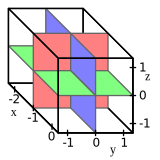
\includegraphics{1_c_echelon_plot_1}} 
\end{center}
%\caption{Part (a), Activity \ref{act:A1.2_7}.}
%\label{Fig:echelon_1}
\end{minipage} %\hspace{0.1in}
\begin{minipage}{1.5in}
\begin{center}
\resizebox{!}{1.5in}{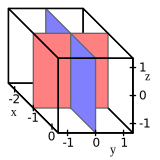
\includegraphics{1_c_echelon_plot_2}} 
\end{center}
%\caption{Part (b), Activity \ref{act:A1.2_7}.}
%\label{Fig:echelon_2}
\end{minipage} %\hspace{0.1in}
\begin{minipage}{1.5in}
\begin{center}
\resizebox{!}{1.5in}{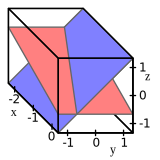
\includegraphics{1_c_echelon_plot_3}}
\end{center}
%\caption{Part (c), Activity \ref{act:A1.2_7}.}
%\label{Fig:echelon_3}
\end{minipage} 
\caption{Figures for Activity \ref{act:1_c_4}.}
\label{F:1_c_1}
\end{center}

\end{figure}

\begin{activity} \label{act:1_c_4} ~
\ba
\item For each part, the reduced row echelon form of the augmented matrix of a system of equations in variables $x$, $y$, and $z$ (in that order) is given. Use the reduced row echelon form to find the solution set to the original system of equations.
	\begin{enumerate}[i.]
	\begin{minipage}{1.4in}
	\item $\left[ \begin{array}{ccc|r} 1 & 0 & 0 & -1 \\ 0 & 1 & 0 & 3 \\ 0 & 0 & 0 & 0 \end{array} \right]$ %(the graph of this system is shown in Figure \ref{Fig:echelon_2})
	\end{minipage}
	\begin{minipage}{1.55in}
	\item $\left[ \begin{array}{ccr|r} 1 & 0 & 2 & -1 \\ 0 & 1 & -1 & 3 \\ 0 & 0 & 0 & 0 \end{array} \right]$ %(the graph of this system is shown in Figure \ref{Fig:echelon_3})
	\end{minipage}
	\begin{minipage}{1.4in}
	\item $\left[ \begin{array}{ccc|r} 1 & 0 & 0 & 2 \\ 0 & 1 & 0 & -1 \\ 0 & 0 & 1 & 3 \end{array} \right]$ %(the graph of this system is shown in Figure \ref{Fig:echelon_1})
	\end{minipage}

\item Each of the three systems above is represented as one of the graphs in Figure \ref{F:1_c_1}. Match each figure with a system.

	\end{enumerate}
	
\item The reduced row echelon form of the augmented matrix of a system of equations in variables $x$, $y$, $z$, and $t$ (in that order) is given. Use the reduced row echelon form to find the solution set to the original system of equations:  
\[\left[ \begin{array}{cccc|r} 1 & 3 & 0 & 0 & -1 \\ 0 & 0 & 1 & 2 & 4 \\ 0 & 0 & 0 & 0 & 1 \end{array} \right].\]



\ea

\end{activity}




\csection{Examples}

\ExampleIntro

\begin{example} Consider the linear system
\begin{align*}
2x_1 + 6x_3 &= x_2 + 2  \\
2x_3 - 4x_1  &=  2x_2\\
x_2 + 4x_3 - 2 &= 2x_1 + 6.
\end{align*}
	\ba
	\item Find the augmented matrix for this system.
	\item Use row operations to find a row echelon form of the augmented matrix of this system.
	\item Use row operations to find the reduced row echelon form of the augmented matrix of this system. 
	\item Find the solution(s), if any, to the system.
	\ea
	
\ExampleSolution Before we can find the augmented matrix of this system, we need to rewrite the system so that the variables are all on one side and the constant terms are on the other side of the equations. Doing so yields the equivalent system
\begin{alignat*}{4}
{2}x_1 	&{}-{}		&{}x_2		&{}+{}	&{6}x_3	&{}={}	& \ 2&{}   \\
{-4}x_1	&{}-{} 		&{2}x_2 		&{}+{}	&{2}x_3	 &{}={} 	& \ 0&{} \\
{-2}x_1	&{}+{}		&{}x_2		&{}+{} 	&{4}x_3	&{}={} 	& \ 8&{.}
\end{alignat*}
Note that this is not the only way to rearrange the system. For example, for the second equation, could be written instead as $4x_1+2x_2-2x_3=0$ to minimize the number of negative signs in the equation. 
\ba
\item The augmented matrix for this system is 
\[\left[ \begin{array}{rrc|c} 2&-1&6&2 \\ -4&-2&2&0 \\ -2&1&4&8 \end{array} \right].\]
\item Our first steps to row echelon form are to eliminate the entries below the leading entry in the first row. To do this we replace row two with row two plus 2 times row 1 and we replace row three with row three plus row one. This produces the row equivalent matrix
\[\left[ \begin{array}{crc|c} 2&-1&6&2 \\ 0&-4&14&4 \\ 0&0&10&10 \end{array} \right].\]
This matrix is now in row echelon form. 
\item To continue to find the reduced row echelon form, we replace row two with row two times $-\frac{1}{4}$ to get a leading 1 in the second row, and we replace row three with row three times $\frac{1}{10}$ to get a leading 1 in the third row and obtain the row equivalent matrix
\[\renewcommand{\arraystretch}{1.4} \left[ \begin{array}{crr|r} 2&-1&6&2 \\ 0&1&-\frac{7}{2}&-1 \\ 0&0&1&1 \end{array} \right].\]
Now we perform backwards elimination to make the entries above the leading $1$s equal to $0$, starting with the third column and working backwards. Replace row one with row one minus $6$ times row three and replace row two with row two plus $\frac{7}{2}$ row three to obtain the row equivalent matrix
\[\renewcommand{\arraystretch}{1.4} \left[ \begin{array}{crc|r} 2&-1&0&-4 \\ 0&1&0&\frac{5}{2} \\ 0&0&1&1 \end{array} \right].\] 
For the second column, we replace row one with row one plus row two to obtain the row equivalent matrix
\[\renewcommand{\arraystretch}{1.4} \left[ \begin{array}{ccc|r} 2&0&0&-\frac{3}{2} \\ 0&1&0&\frac{5}{2} \\ 0&0&1&1 \end{array} \right].\] 
Since the leading entry in row one is not a one, we have one more step before we have the reduced row echelon form. Finally, we replace row one with row one times $\frac{1}{2}$. This gives us the reduced row echelon form
\[\renewcommand{\arraystretch}{1.4} \left[ \begin{array}{ccc|r} 1&0&0&-\frac{3}{4} \\ 0&1&0&\frac{5}{2} \\ 0&0&1&1 \end{array} \right].\] 
\item We can read off the solution to the system from the reduced row echelon form: $x_1 = -\frac{3}{4}$, $x_2 = \frac{5}{2}$, and $x_3 = 1$. You should check in the original equations to make sure we have the correct solution. 
\ea

 \end{example}
 
 \begin{example} In this example, $a$ and $b$ are unknown scalars. Consider the system with augmented matrix 
 \[\left[ \begin{array}{ccc|c} 1&2&a&3 \\ 1&0&0&b \\ 0&1&1&0 \end{array} \right].\] 
 Find all values of $a$ and $b$ so that the system has:
 	\ba
	\item Exactly one solution (and find the solution)
	\item No solutions
	\item Infinitely many solutions (and find all solutions)
	\ea

\ExampleSolution Let $x_1$, $x_2$, and $x_3$ be the variables corresponding to the first, second, and third columns, respectively, of the augmented matrix. To answer these questions, we row reduce the augmented matrix. We interchange rows one and two and then also rows two and three to obtain the matrix
\[\left[ \begin{array}{ccc|c} 1&0&0&b  \\ 0&1&1&0 \\ 1&2&a&3  \end{array} \right].\] 
Now we replace row three with row three minus row one to produce the row equivalent matrix 
\[\left[ \begin{array}{crc|r} 1&0&0&b  \\ 0&1&1&0 \\ 0&2&a&3-b  \end{array} \right].\] 
Next, replace row three with row three minus $2$ times row two. This yields the row equivalent matrix
\[\left[ \begin{array}{ccc|c} 1&0&0&b  \\ 0&1&1&0 \\ 0&0&a-2&3-b  \end{array} \right].\] 
We now have a row echelon form. 
\ba
\item The system will have exactly one solution when the last row has the form $[0 \ 0 \ u \ v]$ where $u$ is not zero. Thus, the system has exactly one solution when $a-2 \neq 0$, or when $a \neq 2$.  In this case, the solution is 
\begin{align*}
x_3 &= \frac{3-b}{a-2}, \\
x_2 &= -x_3 = \frac{b-3}{a-2} \\
x_1 &= b.
\end{align*}
You should check to ensure that this solution is correct. The other cases occur when $a = 2$. 
\item When $a=2$ and $3-b \neq 0$ (or $b \neq 3$), then we have a row of the form $[0 \ 0 \ 0 \ t]$, where $t$ is not $0$. In these cases there are no solutions.
\item When $a=2$ and $b = 3$, then the last row is a row of all zeros. In this case, the system is consistent and $x_3$ is a free variable, so the system has infinitely many solutions. The solutions are 
\begin{align*}
x_1 &= b \\
x_2 &= -x_3 \\
x_3 &\text{ is free.}
\end{align*}
You should check to ensure that this solution is correct.
\ea

 \end{example}

\csection{Summary}

In this section we learned about the row echelon and reduced row echelon forms of a matrix and some of the things these forms tell us about solutions to systems of linear equations. 
\begin{itemize}
\item A matrix is in row echelon form if 
	\begin{enumerate}
    \item All nonzero rows are above any rows of all zeros.
    \item Each \textbf{pivot} (the first nonzero entry) of a row is in a column to the right of the pivot of the row above it.
    \end{enumerate}
\item Once an augmented matrix is in row echelon form, we can use back substitution to solve the corresponding linear system. 
\item To reduce a matrix to row echelon form we do the following: 
	\begin{itemize}
	\item Begin with the leftmost nonzero column (if there is one). This will be a pivot column. 
	\item Select a nonzero entry in this pivot column as a pivot. If necessary, interchange rows to move this entry to the first row (this entry will be a pivot).
	\item Use row operations to create zeros in all positions below the pivot.
	\item Cover (or ignore) the row containing the pivot position and cover all rows, if any, above it. Apply the preceding steps to the submatrix that remains. Repeat the process until there are no more nonzero rows to modify.
	\end{itemize}
\item A matrix is in reduced row echelon form if it is in row echelon form and 
	\begin{enumerate}
    \item[(3)] The pivot in each nonzero row is 1.
    \item[(4)] Each pivot is the only nonzero entry in its column.
	\end{enumerate}
\item To obtain the reduced row echelon form from the row echelon form, beginning with the rightmost pivot and working upward and to the left, create zeros above each pivot. If a pivot is not 1, make it 1 by an appropriate row multiplication.
\item Both row echelon forms of an augmented matrix tell us about the number of solutions to the corresponding linear system.
	\begin{itemize}
	\item A linear system is inconsistent if and only if a row echelon form of the augmented matrix of the system contains a row of the form
    \[[0 \ 0 \ 0 \ \cdots \ 0 \ *],\]
    where $*$ is not zero. Another way to say this is that a linear system is inconsistent if and only if the last column of the augmented matrix of the system is a pivot column.
	\item A consistent linear system will have a unique solution if and only if each column but the last in the augmented matrix of the system is a pivot column. This is equivalent to saying that a consistent linear system will have a unique solution if and only if the consistent system has no free variables.
	\item A consistent linear system will have infinitely many solutions if and only if the coefficient matrix of the system contains a non-pivot column. In that case, the free variables corresponding to the non-pivot columns can be chosen arbitrarily and the basic variables corresponding to pivot columns can be written in terms of the free variables.
	\item A linear system can have no solutions, exactly one solution, or infinitely many solutions.
	\end{itemize}  
\end{itemize}




\csection{Exercises}
\be
\item Represent the following linear system in variables $x_1, x_2, x_3$ in augmented matrix form and use row reduction to find the general solution of the system.
\begin{alignat*}{5}
{}x_1 	&{}+{}	&{}x_2	&{}-{}	&{}x_3 	&= &{}4&{} \\
{}x_1	&{}+{}	&{2}x_2 &{}+{}	&{2}x_3 &= &{}3&{}\\
{2}x_1	&{}+{}	&{3}x_2 &{}-{}	&{3}x_3 &= &{}11&{.}
\end{alignat*}

\item Represent the following linear system in variables $x_1, x_2, x_3$ in augmented matrix form after rearranging the terms and use row reduction to find all solutions to the system. %change numbers to make it nicer. x1=19, x2=3, x3=10 currently
\begin{align*}
x_1 - x_3 - 2x_2 &= 3 \\
2x_3 + 2 &= x_1 +x_2\\
4x_2 + 2x_1 - 2 &= 5x_3.
\end{align*}

\item Check that the reduced row echelon form of the matrix 
\[ \left[ \begin{array}{rrrr} 1 &-1& 3& 2 \\ -1& 2&-4&-1 \\ 2&0&6&8 \end{array} \right] \]
is
\[ \left[ \begin{array}{cccc} 1 &0&0&1 \\ 0&1&0&2 \\ 0&0&1&1 \end{array} \right] \, .\]

\item Consider the following system:
\begin{alignat*}{5}
{}x 	&{}-{} 	&{2}y 	&{}+{} 	&{}z 		&{}={}	&\ {-}&1&{}   \\
{}		&{}		&{2}y	&{}-{} 	&{4}z	&{}={} 	& \ {}&6&{} \\ 
{}		&{}		&{h}y	&{}-{} 	&{2}z	&{}={} 	& \ {}&1&{.} 
\end{alignat*}
	\ba
	\item Find a row echelon form of the augmented matrix for this system.

	\item For which values of $h$, if any, does the system have (i.) no solutions, (ii.) exactly one solution, (iii.) infinitely many solutions? Find the solutions in each case.

	\ea

\item Find the general solution of the linear system corresponding to the following augmented matrix:
\[\left[ \begin{array}{rrcr|r} 1&-1&2&1&2 \\ -1&2&2&-1&-5\\ 1&1&10&2&-1 \end{array}  \right].\]

\item What are the conditions, if any, on the $a, b, c$ values so that the following augmented matrix corresponds to a consistent linear system? How many solutions will the consistent system have? Explain. 
\[\left[ \begin{array}{rrr|c} 1 & 2 & 3 &a \\ 2&3&7&b \\ -1&-4&-1&c \end{array}  \right].\]

\item In this exercise the symbol $\blacksquare$ denotes a non-zero number and the symbol * denotes any real number (including $0$).
\ba
\item Is the augmented matrix 
\[\left[ \begin{array}{cc|c} \blacksquare&*&* \\ 0&\blacksquare&* \end{array} \right]\]
in a form to which back substitution will easily give the solutions to the system?  Explain your reasoning. (Hint: In order to help see what happens in the general case, substitute some numbers in place of the $\blacksquare$'s and *'s and answer the question for that specific system first. Then determine if your answer generalizes.)


\item  The above matrix is a possible form of an augmented matrix with 2 rows and 3 columns corresponding to a linear system after forward elimination, i.e., a linear system for which back substitution will easily give the solutions. Determine the other possible such forms of the nonzero augmented matrices with 2 rows and 3 columns. As in part (a), use the symbol $\blacksquare$ to denote a non-zero number and * to denote any real number.


\ea


\item Give an example of a linear system with a unique solution for which a row echelon form of the augmented matrix of the system has a row of 0's.

\item Come up with an example of an augmented matrix with 0's in the rightmost column corresponding to an inconsistent system, if possible. If not, explain why not.

\item Find two different row echelon forms which are equivalent to the same matrix not given in row echelon form.


\item Determine all possible row echelon forms of a $2\times 2$ matrix. Use the symbol $\blacksquare$ to denote a non-zero number and * to denote a real number with no condition on being 0 or not to represent entries.

\item Label each of the following statements as True or False. Provide justification for your response.
	\ba
	\item \textbf{True/False} The number of pivots of an $m \times n$ matrix cannot exceed $m$. (Note: Here $m$, $n$ are some unknown numbers.)
	\item \textbf{True/False} The row echelon form of a matrix is unique.
	\item \textbf{True/False} The reduced row echelon form of a matrix is unique.
	\item \textbf{True/False} A system of equations where there are fewer equations than the number of unknowns (known as an underdetermined system) cannot have a unique solution.
	\item \textbf{True/False} A system of equations where there are more equations than the number of unknowns (known as an overdetermined system) cannot have a unique solution.
	\item  \textbf{True/False} If a row echelon form of the {\em augmented matrix} of a system of three equations in two unknowns has three pivots, then the system is inconsistent.
	\item \textbf{True/False} If the coefficient matrix of a system has pivots in every row, then the system is consistent.
	\item \textbf{True/False} If there is a row of zeros in a row echelon form of the augmented matrix of a system of equations, the
system has infinitely many solutions.
	\item \textbf{True/False} If there is a row of zeros in a row echelon form of the augmented matrix of a system of $n$ equations in $n$ variables, the system has infinitely many solutions.
	\item \textbf{True/False} If a linear system has no free variables, then the system has a unique solution.
	\item  \textbf{True/False} If a linear system has a free variable, then the system has infinitely many solutions.
	\ea
\ee


\csection{Project: Modeling a Chemical Reaction}

Recall the chemical equation
\begin{equation*}
\text{C}_2\text{H}_6 + \text{O}_2 \to \text{CO}_2 + \text{H}_2\text{O} %\label{eq:reaction1}
\end{equation*}
from the beginning of this section. This equation illustrates the reaction between ethane ($\text{C}_2\text{H}_6$) and oxygen ($\text{O}_2$),called the \emph{reactants}, to produce carbon dioxide ($\text{CO}_2$) and water ($\text{H}_2\text{O}$), called the \emph{products} of the reaction.  In any chemical reaction, the total mass of the reactants must equal the total mass of the products. In our reaction the chemicals involved are made up of carbon (C), hydrogen (H), and oxygen (O) atoms. To balance the equation, we need to know how many molecules of each chemical are combined to preserve the number of atoms of C, H, and O.

Let $x_1$ be the number of molecules of $\text{C}_2\text{H}_6$, $x_2$ the number of molecules of $\text{O}_2$, $x_3$ the number of molecules of $\text{CO}_2$, and $x_4$ the number of molecules of $\text{H}_2\text{O}$ in the reaction. We can then represent this reaction as
\[x_1 \text{C}_2\text{H}_6 + x_2 \text{O}_2 \to x_3 \text{CO}_2 + x_4 \text{H}_2\text{O}.\]

In each molecule (e.g., ethane $\text{C}_2\text{H}_6$), the subscripts indicate the number of atoms of each element in the molecule. So 1 molecule of ethane contains 2 atoms of carbon and 6 atoms of hydrogen. Thus, there are 2 atoms of carbon in $\text{C}_2\text{H}_6$ and 0 atoms of carbon in $\text{O}_2$, giving us  $2x_1$ carbon atoms in $x_1$ molecules of $\text{C}_2\text{H}_6$ and 0 carbon atoms in $x_2$ molecules of $\text{O}_2$. On the product side of the reaction there is 1 carbon atom in $\text{CO}_2$ and 0 carbon atoms in $\text{H}_2\text{O} $. To balance the reaction, we know that the number of carbon atoms in the products must equal the number of carbon atoms in the reactants. 

\begin{pactivity} \label{act:1_c_reaction_1} ~
	\ba
	\item Set up an equation that balances the number of carbon atoms on both sides of the reaction.

	\item Balance the numbers of hydrogen and oxygen atoms in the reaction to explain why
\begin{align*}
6x_1 &= 2x_4 \\
2x_2 &= 2x_3 + x_4.
\end{align*}

	\item So the system of linear equations that models this chemical reaction is  \begin{alignat*}{5}
{2}x_1 	&{}		&{}		&{}-{}	&{}x_3	&{}		&{} 			&{}={}	& \ 0&{}   \\
{6}x_1	&{} 		&{} 		&{}		&{}		&{}-{}	&{2}x_4 	&{}={} 	& \ 0&{} \\
{}			&{}		&{2}x_2	&{}-{} 	&{2}x_3	&{}-{}	&{}x_4		&{}={} 	& \ 0&{.}
\end{alignat*}

Find all solutions to this system and then balance the reaction. Note that we cannot have a fraction of a molecule in our reaction.  (Hint: Some of the work needed is done in Preview Activity \ref{pa:1_c}.) 
	\ea

\end{pactivity}

\begin{pactivity} Chemical reactions can be very interesting. 
\ba
\item Carbon dioxide, $\text{CO}_2$, is a familiar product of combustion. For example, when we burn glucose, $\text{C}_6\text{H}_{12}\text{O}_6$, the products of the reaction are carbon dioxide and water:
\begin{equation}
\text{C}_6\text{H}_{12}\text{O}_6 + \text{O}_2 \to \text{CO}_2 + \text{H}_2\text{O}.\label{eq:reaction2}
\end{equation}
Use the techniques developed in this project to balance this reaction.

\item To burn glucose, we need to add oxygen to make the combustion happen. Carbon dioxide is different in that it can burn without the presence of oxygen. For example, when we mix magnesium (Mg) with dry ice ($\text{CO}_2$), the products are magnesium oxide (MgO) and carbon (C). This is an interesting reaction to watch: you can see it at many websites, e.g.,
\url{http://www.ebaumsworld.com/video/watch/404311/} or 
\url{https://www.youtube.com/watch?v=-6dfi8LyRLA}.

Use the method determined above to balance the chemical reaction 
\begin{equation}
\text{Mg} + \text{CO}_2 \to \text{MgO} + \text{C}. \label{eq:reaction3}
\end{equation}

\ea

\end{pactivity}



